\documentclass[10pt]{article}
% Layout close to the NeurIPS / AI4Mat workshop format (5.5 x 9 in text block, Times).
% To use an official style file instead, delete the geometry/mathptmx lines and add e.g.
% \usepackage[preprint]{neurips_2025}.
\usepackage[letterpaper,textwidth=5.5in,textheight=9in,top=1in,headheight=12pt,headsep=25pt,footskip=30pt]{geometry}
\usepackage[T1]{fontenc}
\usepackage[utf8]{inputenc}
\usepackage{mathptmx}
\usepackage{amsmath,amssymb}
\usepackage{microtype}
\usepackage{booktabs}
\usepackage{graphicx}
\usepackage{xcolor}
\usepackage[numbers,sort&compress]{natbib}
\usepackage[small,labelfont=bf]{caption}
\usepackage{enumitem}
\usepackage{multirow}
\usepackage[colorlinks=true,linkcolor=blue!50!black,citecolor=blue!50!black,urlcolor=blue!50!black]{hyperref}
\setlist{nosep,leftmargin=1.4em}

% Set to 1 for a double-blind submission (hides authors and the repository link).
\newcommand{\anonymous}{0}
\newcommand{\repo}{\ifnum\anonymous=1 [link withheld for review]\else\url{https://github.com/chilalaabubakar/IDL-PROJECT}\fi}

\newcommand{\Dm}{D1$^{-}$}
\newcommand{\Dp}{D1$^{+}$}
\newcommand{\pmsd}[2]{#1\,{\scriptsize$\pm$\,#2}}

\title{Placing Defects Where You Ask:\\ Location-Specific Defect Generation in a Model Glass\\ with Conditional Diffusion}

\ifnum\anonymous=1
\author{Anonymous authors}
\else
\author{
  Stacy Cheruto \quad Nicholaus Ladislaus \quad Abubakar Chilala\\ Gentille Uwera \quad Michel Sangwa\\[2pt]
  Language Technologies Institute, Carnegie Mellon University\\
  {\small\texttt{\{ccheruto, eladisla, achilala, guwera, sbmichel\}@andrew.cmu.edu}}
}
\fi
\date{}

\begin{document}
\maketitle

\begin{abstract}
Defects control many properties of amorphous materials, but obtaining a specific defect at a chosen location still means waiting for it to form in a slow melt-quench simulation or inserting it by hand. Diffusion models now generate realistic amorphous structures, yet they cannot be asked for a particular defect at a particular place. We treat this as conditional generation on periodic point clouds. In a two-dimensional Kob--Andersen glass, a periodic E($n$)-equivariant denoiser receives pinned atoms and a per-atom defect label, uses classifier-free guidance, and regenerates a disk around a requested site inside an existing glass. Every sample is relaxed before it is scored, and its surroundings are compared with those of naturally formed defects. Averaged over three training runs, the model places under-coordinated defects 3.5$\times$ as often as hand insertion (0.22 vs.\ 0.06) with near-natural surroundings, and B-rich defects 1.5--2.4$\times$ as often (0.45--0.71 vs.\ 0.30) with surroundings as natural or more natural. Local melt-quench of the same disk almost never succeeds. Over-coordinated defects fail for every method, and we show that nothing local can hold them. The ranking survives every evaluation setting we varied. Along the way we find that the sampler's step count acts as a cooling rate, that training on the full noise range the sampler visits decides whether generated defects survive relaxation, and that training runs with the same validation loss differ in their effective guidance strength.
\end{abstract}

\section{Introduction}

A defect's behaviour in a glass depends on its surroundings, so studies of plasticity, relaxation or optical properties need many realistic examples of a given defect. Today these come from two sources: melt-quench molecular dynamics (MD), where one waits for the defect to form by chance at an uncontrolled place, and hand insertion, where atoms are moved or replaced and the structure relaxed, which can leave artificial surroundings. Generative models offer a third route. DM2~\citep{yang2026dm2} denoises random atomic positions into amorphous silica and metallic glasses whose structure and properties match MD, at a fraction of the cost for slow cooling rates. Like most generative models for materials~\citep{xie2022cdvae,jiao2023diffcsp,zeni2025mattergen,finkler2026inverse,kwon2024spectroscopy}, it conditions on global quantities. It cannot be asked for a particular local feature at a particular place.

We frame location-specific defect generation like image inpainting~\citep{lugmayr2022repaint}: the defect is fixed, and the model generates realistic surroundings. Two points shape the study.
\begin{itemize}
\item \emph{Location must mean something.} ``At a chosen location'' is trivial in an empty periodic box, since any naturally formed defect can be translated to any point. Our headline task therefore regenerates a disk around a requested site \emph{inside an existing glass}, with everything outside the disk held fixed (Task~B). This is the setting of host-guided inpainting for crystals~\citep{zhong2025inpainting} and of linker design between fixed fragments~\citep{igashov2024difflinker}.
\item \emph{Success must survive physics.} A generated defect counts only if it is still there after the whole structure has been relaxed to a local energy minimum. Realism is measured against naturally formed defects of the same class, with a natural-vs.-natural floor as the reference.
\end{itemize}

\paragraph{Contributions.}
\begin{enumerate}
\item A task and evaluation protocol for location-specific defect generation in glasses: host-conditioned inpainting, success after relaxation, local realism against natural defects, and an MD baseline that re-melts the same disk.
\item A conditional periodic EGNN with pinned atoms, per-atom defect labels and classifier-free guidance~\citep{ho2022cfg}. It beats hand insertion and local melt-quench for two of three defect classes, and the result holds across evaluation settings, re-sampling and three training seeds.
\item Lessons for diffusion models of glasses:
  \begin{itemize}
  \item the number of sampler steps acts as a cooling rate;
  \item the training noise range must cover the sampler's starting noise;
  \item training runs differ in effective guidance strength, which the denoising loss does not show;
  \item equivariance matters more than validation loss for sample quality;
  \item over-coordinated defects are held by their host beyond a radius of 3.5$\sigma$, so no local method can place them.
  \end{itemize}
\end{enumerate}
Figure~\ref{fig:overview} summarises the study.

\begin{figure}[t]
\centering
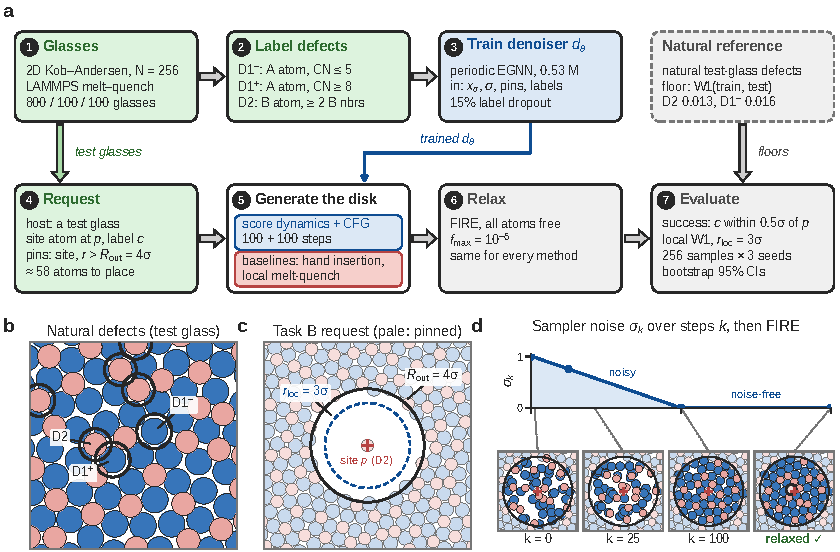
\includegraphics[width=\linewidth]{figures/fig1_overview.pdf}
\caption{Study overview. \textbf{(a)}~Workflow: labelled melt-quench glasses (1--2) train a periodic EGNN denoiser conditioned on pins and per-atom labels (3); a request (4) is answered by guided score dynamics or a baseline (5), relaxed with all atoms free (6) and scored against natural defects (7). \textbf{(b)}~Natural defects (rings) in a test glass; A atoms blue, B atoms pink and smaller. \textbf{(c)}~A real Task~B request: pinned atoms (pale, including the site atom under the cross), the regenerated disk ($R_\text{out}$) and the realism window ($r_\text{loc}$). \textbf{(d)}~The model ($w=6$) answering it: free atoms start uniform in the disk and are denoised as $\sigma_k$ falls; after relaxation the requested D2 (ring) is at the site.}
\label{fig:overview}
\end{figure}

\section{Related work}

\paragraph{Diffusion models for materials.} Denoising diffusion and score-based models~\citep{ho2020ddpm,song2021sde} now generate crystals~\citep{xie2022cdvae,jiao2023diffcsp,zeni2025mattergen} and disordered solids. For amorphous materials, DM2~\citep{yang2026dm2} learns to remove Gaussian displacements from glass configurations and samples by a noisy relaxation it calls score dynamics. It conditions on the cooling rate and reproduces structure and mechanical properties of silica and metallic glasses. Other work conditions on spectra~\citep{kwon2024spectroscopy} or target properties~\citep{finkler2026inverse}. All of these control global quantities; none places a chosen local motif at a chosen site.

\paragraph{Local control.} In images, RePaint~\citep{lugmayr2022repaint} inpaints a masked region with an unconditional model, and guidance~\citep{dhariwal2021,ho2022cfg} strengthens a condition at sampling time. In materials and molecules, the closest settings are host-guided inpainting for crystal structure prediction~\citep{zhong2025inpainting}, constrained diffusion that relaxes crystals containing given point defects~\citep{cui2026constrained}, and linker generation between fixed molecular fragments~\citep{igashov2024difflinker}. A glass differs from these in two ways. There is no lattice to define a defect against, so a defect is a local motif that also occurs naturally. And realism can only be judged statistically, against the ensemble of naturally formed motifs. Our evaluation is built around both points.

\paragraph{Equivariant denoisers.} We use the E($n$)-equivariant EGNN~\citep{satorras2021egnn} as the main backbone. A message-passing network~\citep{gilmer2017mpnn} and a flat MLP serve as less symmetric ablations. Higher-order equivariant networks such as NequIP~\citep{batzner2022nequip}, used by DM2 for silica, are the natural choice in 3D.

\section{Setup}

\paragraph{Glass and defects.} We use the two-dimensional Kob--Andersen binary Lennard-Jones mixture~\citep{kob1995,bruning2009}:
\begin{itemize}
\item 65:35 A:B, density 1.2, $N=256$ atoms in a periodic square box of side 14.6$\sigma$;
\item glasses made in LAMMPS~\citep{thompson2022lammps} by melting at $T=2.0$ for 100$\tau$, quenching at $10^{-2}$ per $\tau$ to $T=0.01$ and minimising the energy;
\item 800 training, 100 validation and 100 test glasses, each screened for crystallinity.
\end{itemize}

Defects are defined by cutoff coordination, with the first shell within $1.4\,\sigma_{\alpha\beta}$:
\begin{itemize}
\item \textbf{\Dm}: an A atom with at most 5 neighbours (1.7 per glass);
\item \textbf{\Dp}: an A atom with at least 8 neighbours (1.4 per glass);
\item \textbf{D2}: a B atom with at least two B neighbours within $1.2\sigma$ (10 per glass).
\end{itemize}
Thresholds are frozen on the training split.

\paragraph{Tasks.} In \textbf{Task~B} (headline), a test glass supplies the host. The requested site $p$ is the host atom of the defect's species nearest a random point. That atom, which carries the label, and every atom farther than $R_\text{out}=4\sigma$ from it are pinned; the $\approx$58 atoms in between are regenerated, starting from uniform random positions. \textbf{Task~A} generates a whole box with the defect at its centre. It is reported for completeness, since location is trivial there.

\paragraph{Model.} The denoiser is an EGNN~\citep{satorras2021egnn} made periodic with minimum-image edge vectors:
\begin{itemize}
\item 4 layers, width 128, cutoff 2.5$\sigma$, 0.53\,M parameters;
\item node inputs: species, random Fourier features of $\log\sigma$, a pinned flag, and a defect-label token (``none'' everywhere except the requested site);
\item output: a displacement per atom, zeroed on pinned atoms.
\end{itemize}

Training follows DM2's formulation~\citep{yang2026dm2}. Positions are perturbed as $x_\sigma = x_0 + \sigma\epsilon$ with $\epsilon\sim\mathcal{N}(0,I)$ (pinned atoms untouched), and the denoiser $d_\theta$ regresses the added displacement on the unpinned atoms $U$:
\begin{equation}
\mathcal{L}(\theta) = \mathbb{E}_{x_0,\sigma,\epsilon,m,c}\Big[\tfrac{1}{|U|}\textstyle\sum_{i\in U}\big\|d_\theta(x_\sigma,\sigma,m,c)_i-\sigma\epsilon_i\big\|^2\Big],
\label{eq:loss}
\end{equation}
where $m$ is the pin mask and $c$ the per-atom labels. Further details:
\begin{itemize}
\item $\sigma \sim \mathcal{U}(10^{-3}, \sigma_\text{max})$;
\item training requests mix whole-box, patch and host-inpainting modes (probabilities 0.5 / 0.3 / 0.2), centred on a natural defect half of the time;
\item labels are dropped with probability 0.15 for classifier-free guidance;
\item AdamW, learning rate $2\times10^{-4}$, batch 16, 50{,}000 updates, EMA 0.999; about 4\,h on one T4 GPU.
\end{itemize}
Two recipes differ only in $\sigma_\text{max}$: 0.5 (DM2's choice of half a bond length; used for \Dm{} and Task~A) and 1.0 (Section~\ref{sec:why}; used for D2).

\paragraph{Sampler.} DM2's score dynamics alternates denoising with fresh noise,
\begin{equation}
x_{k+1} = x_k - \tilde d(x_k,\sigma_k) - \eta_k,\qquad \eta_k\sim\mathcal{N}(0,s_k^2 I),\quad s_k\sim\mathcal{U}(10^{-3},\sigma_k),
\label{eq:sampler}
\end{equation}
with pinned atoms reset after every step. Classifier-free guidance~\citep{ho2022cfg} combines the conditional and label-free predictions,
\begin{equation}
\tilde d = (1+w)\,d_\theta(x,\sigma,m,c) - w\,d_\theta(x,\sigma,m,\varnothing),
\label{eq:cfg}
\end{equation}
so $w=0$ is the unguided conditional model. Settings:
\begin{itemize}
\item 100 steps with $\sigma_k$ falling linearly from 1.0 to $10^{-3}$, then 100 noise-free steps;
\item $\sigma$ passed to the model is clipped at its training $\sigma_\text{max}$.
\end{itemize}

\paragraph{Baselines.}
\begin{itemize}
\item \emph{Chance}: inpainting the same disk without a label.
\item \emph{Hand insertion} (current practice): a natural defect patch of radius 1.5$\sigma$, drawn from the training split, is pasted at the site; each patch atom replaces the nearest host atom of its species.
\item \emph{Local melt-quench}: in LAMMPS, atoms beyond $R_\text{out}$ are frozen, the disk is melted at $T=2.0$ and quenched at the dataset rate, i.e.\ waiting for the defect, confined to the disk.
\item For Task~A: \emph{Clamp} and \emph{RePaint}~\citep{lugmayr2022repaint} with an unconditional model.
\end{itemize}

\paragraph{Evaluation.}
\begin{itemize}
\item \textbf{Relaxation.} Every sample is relaxed with FIRE~\citep{bitzek2006fire} ($f_\text{max}=10^{-6}$), with all atoms free, host included.
\item \textbf{Success.} The atom of the requested species nearest the site lies within $r_\text{tol}=0.5\sigma$ of it and carries the requested label.
\item \textbf{Local realism.} The Wasserstein-1 distance (W1) between the per-atom energies in a window of radius $r_\text{loc}=3\sigma$ around the site and those around natural defects of the same class in the test glasses. The floor is natural training defects against natural test defects: \Dm{} 0.016, \Dp{} 0.018, D2 0.013.
\item \textbf{Statistics.} 256 samples per row, with 95\% bootstrap confidence intervals (CIs) over samples.
\end{itemize}

\begin{figure}[t]
\centering
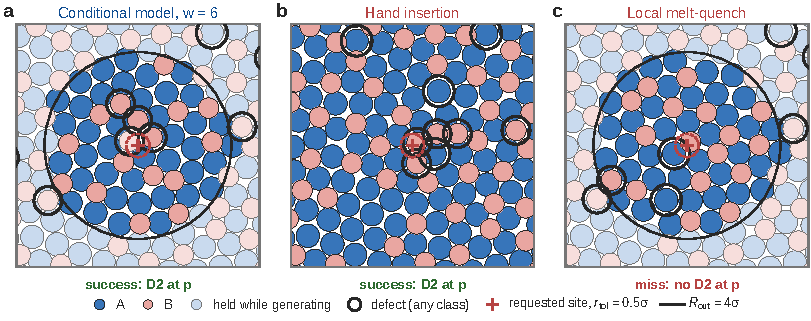
\includegraphics[width=\linewidth]{figures/fig2_taskB.pdf}
\caption{The request of Figure~\ref{fig:overview}c answered by each method, after relaxation ($\pm5\sigma$ around the site; dashed circle: $r_\text{tol}$). Pale atoms were held fixed while generating; rings mark every defect. \textbf{(a)}~The model places a B atom with two B neighbours at the site. \textbf{(b)}~Hand insertion also succeeds here, but its surroundings are far from natural on average (Table~\ref{tab:main}). \textbf{(c)}~Local melt-quench re-forms the disk without a D2 at the site. Of the six requests drawn for these figures, the model answered two, hand insertion four and local melt-quench one; Table~\ref{tab:main} gives rates over 256 requests per seed.}
\label{fig:taskB}
\end{figure}

\section{Results}

\subsection{Main result: defects inside existing glasses}

Table~\ref{tab:main} and Figure~\ref{fig:seeds} give the Task~B results. Model rows are means $\pm$ standard deviations over three training runs (seeds 0--2), each with 256 samples.

\begin{table}[t]
\centering
\caption{Task~B, success after relaxation and local realism (W1 of per-atom energy in a $3\sigma$ window; lower is more natural). Model rows: mean $\pm$ s.d.\ over three training runs; baselines: estimate with 95\% CI. D2 uses the $\sigma_\text{max}=1.0$ recipe, \Dm{} and \Dp{} the $\sigma_\text{max}=0.5$ recipe. $^\dagger$2{,}900-step sampler. $^\ddagger$Seed 0 only.}
\label{tab:main}
\small
\setlength{\tabcolsep}{4pt}
\begin{tabular}{lccccc}
\toprule
& \multicolumn{2}{c}{D2 (B-rich)} & \multicolumn{2}{c}{\Dm{} (under-coordinated)} & \Dp{} \\
\cmidrule(lr){2-3}\cmidrule(lr){4-5}\cmidrule(lr){6-6}
Method & success & local W1 & success & local W1 & success \\
\midrule
Chance (no label)$^\dagger$ & 0.03 & 0.062 & 0.02 & 0.053 & 0.00 \\
Local melt-quench & 0.05 {\scriptsize[0.03, 0.08]} & 0.065 & 0.00 {\scriptsize[0.00, 0.00]} & 0.024 & 0.01 \\
Hand insertion & 0.30 {\scriptsize[0.24, 0.36]} & 0.087 & 0.06 {\scriptsize[0.04, 0.09]} & 0.032 & 0.02 \\
\midrule
Model, $w=2$ & \pmsd{0.45}{0.11} & \pmsd{\textbf{0.051}}{0.006} & \pmsd{\textbf{0.22}}{0.02} & \pmsd{\textbf{0.022}}{0.002} & 0.03$^\ddagger$ \\
Model, $w=6$ & \pmsd{\textbf{0.71}}{0.08} & \pmsd{0.072}{0.016} & \pmsd{0.21}{0.04} & \pmsd{0.038}{0.004} & 0.04$^\ddagger$ \\
\midrule
Natural floor & --- & 0.013 & --- & 0.016 & --- \\
\bottomrule
\end{tabular}
\end{table}

\paragraph{The model beats both baselines on the two classes that can be placed.}
\begin{itemize}
\item \textbf{D2.} At $w=6$ the model succeeds 2.4$\times$ as often as hand insertion on average (2.1--2.7$\times$ per seed), with surroundings as natural or more natural. At $w=2$ it succeeds 1.5$\times$ as often (1.2--1.9$\times$) with clearly more natural surroundings for every seed (W1 0.045--0.056 vs.\ 0.087).
\item \textbf{\Dm.} The model succeeds 3.5$\times$ as often as hand insertion at $w=2$, with surroundings 1.2--1.5$\times$ the natural floor.
\item \textbf{Local melt-quench} almost never produces the defect at the site. Re-forming a 60-atom disk at the dataset's cooling rate is the ``wait for it'' approach in miniature, and rare defects remain rare.
\item \textbf{Cost.} Per success the model needs 1--4 GPU-seconds. That is comparable with hand insertion, whose cost is almost all relaxation (0.8--3.6\,s), and far below local melt-quench (65 wall-clock seconds per D2 success, and no \Dm{} success at all).
\end{itemize}

\paragraph{Guidance trades realism for success.} Stronger guidance places the defect more often before relaxation: D2 0.86 at $w=2$ against 1.00 at $w=6$ (seed 0). More of those placements also survive relaxation, but the surroundings move away from natural. For \Dm{}, success saturates at $w=2$: extra guidance puts more defects in place before relaxation (0.85 at $w=6$), but they sit in shallow basins and relax away. Without guidance ($w=0$) success drops (\Dm{} 0.09 vs.\ 0.23, D2 0.24 vs.\ 0.30 at 300 steps; Appendix~\ref{app:extra}).

\paragraph{\Dp{} fails for every method, and the reason is not local.} Natural \Dp{} sites survive noise followed by relaxation in their own glass. Yet when a natural \Dp{} is transplanted into a host together with its 47 nearest atoms (radius 3.5$\sigma$), it relaxes away 97\% of the time (Appendix~\ref{app:stability}). An over-coordinated atom is held in place by its host beyond 3.5$\sigma$, so neither a patch nor a pinned label can carry it.

\begin{figure}[t]
\centering
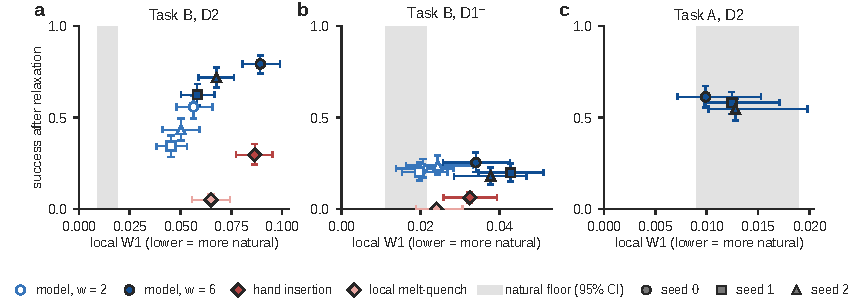
\includegraphics[width=\linewidth]{figures/fig3_seeds.pdf}
\caption{Success against local W1 for each training seed (marker shape), guidance weight (open: $w=2$, filled: $w=6$) and baseline (red diamonds); grey band: natural floor (95\% CI). For D2, the seeds at each $w$ lie along the same success--realism line that guidance traces. Seed~0, behind all earlier D2 numbers, is the most successful.}
\label{fig:seeds}
\end{figure}

\subsection{Why generated defects survive relaxation, or do not}
\label{sec:why}

A natural defect survives Gaussian noise of mean displacement up to $\approx$0.19$\sigma$ followed by relaxation 99--100\% of the time (Appendix~\ref{app:stability}). Generated samples move 0.16--0.24$\sigma$ during relaxation, yet only 25--80\% of their placed defects survive. The gap is the generator's: its defects sit in shallower basins than natural ones.

Table~\ref{tab:noise} shows the main lever. Following DM2, our original recipe trains with noise up to half a bond length ($\sigma_\text{max}=0.5$), while the sampler starts at $\sigma=1$, a range the model never saw. Retraining with $\sigma_\text{max}=1.0$ makes the model place the D2 defect more reliably before relaxation, and keep it more often afterwards: 79\% instead of 57\% at $w=6$. D2 success rises from 0.54 to 0.79 (seed 0). For \Dm{} the original recipe remains slightly better (0.22 vs.\ 0.21 at $w=2$, 0.25 vs.\ 0.22 at $w=6$), so we report each class with its better recipe.

\begin{table}[t]
\centering
\caption{Training noise range (Task~B, D2, seed 0). ``Kept'' = success after / before relaxation.}
\label{tab:noise}
\small
\begin{tabular}{lccccc}
\toprule
Recipe & $w$ & placed (before relax) & success (after) & kept & local W1 \\
\midrule
$\sigma_\text{max}=0.5$ & 2 & 0.67 & 0.35 & 52\% & 0.040 \\
$\sigma_\text{max}=0.5$ & 6 & 0.94 & 0.54 & 57\% & 0.064 \\
$\sigma_\text{max}=1.0$ & 2 & 0.86 & 0.56 & 65\% & 0.056 \\
$\sigma_\text{max}=1.0$ & 6 & 1.00 & 0.79 & 79\% & 0.089 \\
\bottomrule
\end{tabular}
\end{table}

\subsection{Robustness}

\paragraph{Reproducibility and training seeds.} Re-running the nine headline rows with the same seed reproduced eight of them to the last digit; the ninth moved within its CI. A fresh evaluation draw (new hosts, sites and noise) moved success by 0.02 on average, within the bootstrap CIs. Across three training runs:
\begin{itemize}
\item \Dm{} and Task~A vary no more than the evaluation noise (s.d.\ 0.02--0.04).
\item Task~B D2 varies twice as much (s.d.\ 0.08--0.11; Figure~\ref{fig:seeds}).
\item The D2 seeds rank identically in success and in local W1, and their placement rate before relaxation differs (0.41--0.86 at $w=2$). Their validation losses agree to within a few percent.
\item So each training run ends with a different \emph{effective guidance strength}, invisible to the denoising loss.
\item The model beats both baselines for every seed, with one exception: seed~1 at $w=2$, whose success CI overlaps hand insertion's while its surroundings remain clearly more natural.
\end{itemize}

\paragraph{Evaluation settings.} We moved each setting on its own (Figure~\ref{fig:sens}): the defect cutoffs by $\pm0.05$ (relabelling the natural references to match), the success radius by $\pm0.1\sigma$, the realism window by $\pm0.5\sigma$, and the regenerated disk $R_\text{out}$ to 3 and 5$\sigma$. The results:
\begin{itemize}
\item The ranking never changes. Absolute success moves by up to $\approx$0.1 with the definitions, so rates must be quoted with the definition used.
\item Hand insertion's damage is local: its W1 falls from 0.113 to 0.068 as the window grows. The model's is spread over the regenerated disk, and its W1 at $w=6$ stays at 0.089. Realism comparisons should therefore be shown at more than one window size.
\item Success changes little with $R_\text{out}$ (all changes within the CIs), although the model was trained at 4$\sigma$ only.
\item A larger disk makes D2 surroundings much more natural (W1 0.026 at $R_\text{out}=5$, $w=2$). This may partly reflect the boundary between regenerated and pinned atoms moving out of the window.
\end{itemize}

\begin{figure}[t]
\centering
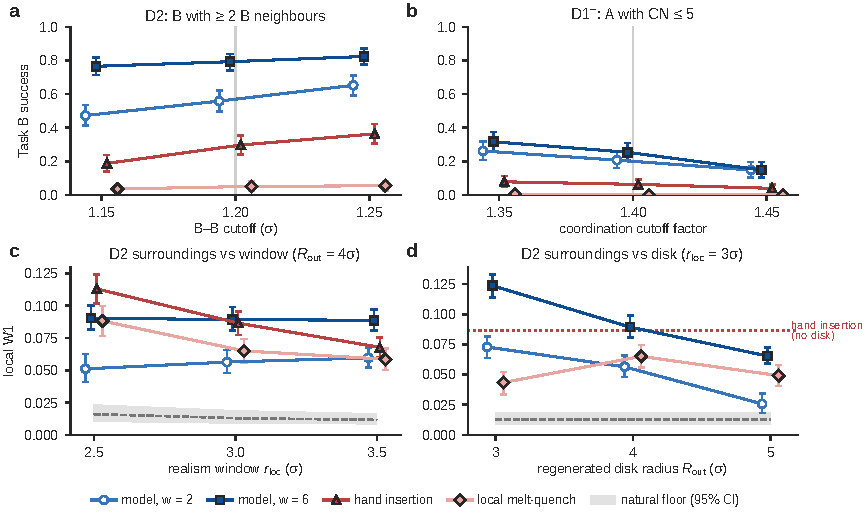
\includegraphics[width=\linewidth]{figures/fig4_sensitivity.pdf}
\caption{Sensitivity (seed 0, Task~B). \textbf{(a, b)}~Success against the defect cutoff for D2 and \Dm{} (grey line: frozen value). \textbf{(c, d)}~D2 local W1 against the realism window and the regenerated-disk radius; grey band: natural floor. The method ranking holds everywhere; hand insertion's damage is local (c), and a larger disk gives more natural surroundings (d).}
\label{fig:sens}
\end{figure}

\subsection{Lessons for diffusion models of glasses}

\paragraph{The step count is a cooling rate.} The score-dynamics sampler adds fresh noise at every step, so a longer schedule is a slower anneal (Table~\ref{tab:steps}, Appendix~\ref{app:extra}). DM2's default of 3{,}000 steps over-anneals our glass: lower energy than the training glasses, fewer B--B contacts, worse $g(r)$. 100 steps reproduce the natural energy at a fifteenth of the cost, without changing Task~B success.

The same issue appears, in the other direction, when we rerun DM2's pretrained amorphous-silica model with its own settings (Appendix~\ref{app:stage0}). Its samples have the right tetrahedra and $g(r)$ peaks, but their disorder matches a glass cooled 100$\times$ faster than the training data. The cooling rate of generated glass should be measured, not assumed.

\paragraph{Whole generated glasses are chemically biased.} Even at 100 steps, generated boxes have about two-thirds of the natural B--B contacts, and $g_{AB}$ stays at 3.5$\times$ the floor. Widening the noise range does not change this (0.34 vs.\ 0.36). This is why Task~B, which keeps most of a natural host, is the more trustworthy setting. In Task~A the model still reaches D2 success \pmsd{0.58}{0.03} over three seeds with surroundings at the natural floor (W1 \pmsd{0.012}{0.002}), against 0.34--0.35 for Clamp and RePaint patches.

\paragraph{Symmetry matters more than loss.} At $N=64$ we trained three unconditional denoisers with the same recipe (Table~\ref{tab:ladder}, Appendix~\ref{app:extra}). The EGNN (permutation and rotation equivariant) makes the most natural glasses. A message-passing network~\citep{gilmer2017mpnn} (permutation only) reaches a \emph{lower} validation loss but worse samples. A flat MLP on the coordinates does not learn at all (validation loss at the predict-zero level), and 16\% of its samples are partly crystalline.

\section{Discussion and limitations}

The question was whether a diffusion model can be asked for a specific defect at a specific place, with surroundings that look natural. For two of three defect classes in a model glass, the answer is yes, and more reliably than the methods used today. The failure is informative: an over-coordinated atom is stabilised by its host beyond any local patch, so it marks a limit for every local placement method, not just ours.

The main lessons concern how such models should be built and evaluated: cover the noise range the sampler visits, calibrate the step count against the cooling rate, judge samples after relaxation and against natural references, and report several training runs, since runs with the same loss can differ in how strongly they follow the condition.

\paragraph{What this means in practice.}
\begin{itemize}
\item \textbf{Choosing a method.} When many instances of a local motif are needed in realistic surroundings, the conditional model gives 1.5--3.5$\times$ more correct placements per attempt than hand insertion, with surroundings closer to natural. Hand insertion remains the cheapest per attempt and is adequate when the surroundings do not matter. Re-melting a region is not a practical way to obtain a specific defect.
\item \textbf{Guidance is a dial.} The guidance weight trades success against realism (Figure~\ref{fig:seeds}). Since each trained model sits at its own point on that curve, the weight should be chosen per model, for a target realism or success rate, rather than fixed in advance.
\item \textbf{Non-local defects need non-local regeneration.} A defect stabilised by its host beyond 3.5$\sigma$, like \Dp{}, cannot be carried by a patch or a label on one atom. Regenerating a larger region, or conditioning on a descriptor of the wider host, are the obvious next tests. The improvement in realism at larger $R_\text{out}$ suggests the model can use a larger region.
\item \textbf{The evaluation transfers.} Checking success after relaxation, comparing with natural floors and reporting several seeds and settings apply to any generative model for disordered matter. Each of them changed a conclusion in this study.
\end{itemize}

\paragraph{Limitations.} The system is a two-dimensional model glass of 256 atoms, and defects are defined geometrically, not by a property. Whole generated glasses are chemically biased. D2 success varies between training runs; choosing the guidance weight per trained model on validation data may reduce this spread, which we have not tested. Because MD is cheap in 2D, cost is not a decisive argument here.

\paragraph{Outlook.} We are extending the approach to three-dimensional amorphous silica with a NequIP-type denoiser~\citep{batzner2022nequip} and DM2's data and potential~\citep{bouhadja2013}. The targets, coordination defects, non-bridging oxygens and small rings, are rare in slowly cooled glass, which is where a generator that can place them is most useful. An independent machine-learned potential will check that generated and natural defects are physically equivalent.

\section{Conclusion}

Conditional diffusion with pinned atoms, per-atom labels and guidance places requested defects inside existing glasses more often than hand insertion or local melt-quench. Their surroundings are close to those of naturally formed defects, and the result holds across evaluation settings and training runs. The same study shows that sampler length, training noise range and training seed all affect what a diffusion model of a glass produces, and that each needs to be measured rather than assumed.

\paragraph{Code and data.} Code, generated datasets, trained weights and every result in this paper: \repo.

\ifnum\anonymous=0
\paragraph{Acknowledgements.} This work was carried out as a course project in Introduction to Deep Learning at Carnegie Mellon University. Experiments ran on Google Colab and Kaggle GPUs.
% AI-use statement: add here if the venue requires one.
\fi

\bibliographystyle{unsrtnat}
\bibliography{refs}

\appendix
\section{Additional results}
\label{app:extra}

\paragraph{Guidance sweep (Task~B, seed 0, 300 steps, $\sigma_\text{max}=0.5$).} The table gives success after relaxation, with placement before relaxation in brackets.

\begin{center}\small
\begin{tabular}{lccccc}
\toprule
$w$ & 0 & 1 & 2 & 4 & 6 \\
\midrule
\Dm{} success (placed) & 0.09 (0.19) & 0.17 (0.46) & 0.23 (0.59) & 0.21 (0.77) & 0.23 (0.85) \\
D2 success (placed) & 0.24 (0.32) & 0.31 (0.58) & 0.30 (0.73) & 0.47 (0.80) & 0.56 (0.97) \\
\bottomrule
\end{tabular}
\end{center}

\paragraph{Task~A (seed 0, 100 steps).} Success after relaxation, with local W1 in brackets.

\begin{center}\small
\begin{tabular}{lccc}
\toprule
Method & D2 & \Dm{} & \Dp{} \\
\midrule
Unconditional (chance) & 0.01 (0.055) & 0.00 (0.069) & 0.00 \\
Clamp patch & 0.34 (0.022) & 0.01 (0.053) & 0.04 \\
RePaint patch ($U=1$) & 0.35 (0.045) & 0.02 (0.042) & 0.04 \\
Model $w=6$, $\sigma_\text{max}=0.5$ & 0.61 (0.010) & 0.23 (0.034) & 0.05 \\
Model $w=6$, $\sigma_\text{max}=1.0$ & 0.84 (0.046) & 0.16 (0.092) & 0.01 \\
\bottomrule
\end{tabular}
\end{center}

RePaint resampling ($U=5, 10$) does not help on this sampler: every resampling pass re-runs part of the noisy schedule, so it acts as extra annealing (energy $-3.704$ and $-3.712$).

\begin{table}[h]
\centering
\caption{Unconditional whole-box samples (seed 0) against sampler steps. Natural test glasses: energy $-3.681$, $g_{AB}$ floor 0.067, 0.56 B--B contacts per B atom.}
\label{tab:steps}
\small
\begin{tabular}{lcccc}
\toprule
noisy steps & 100 & 300 & 900 & 2{,}900 (DM2) \\
\midrule
energy per atom & $-3.678$ & $-3.692$ & $-3.706$ & $-3.720$ \\
$g_{AB}(r)$ L1 & 0.23 & 0.30 & 0.39 & 0.49 \\
B--B contacts per B & 0.36 & 0.31 & 0.25 & --- \\
\bottomrule
\end{tabular}
\end{table}

\begin{table}[h]
\centering
\caption{Symmetry ladder at $N=64$ (unconditional, 100 steps, relaxed). Natural: energy $-3.636$, $g_{AB}$ floor 0.094, 0.475 B--B per B, local W1 floor 0.007.}
\label{tab:ladder}
\small
\begin{tabular}{lcccccc}
\toprule
Model & energy & $g_{AB}$ L1 & B--B per B & local W1 & crystallised & val.\ loss / $\sigma^2$ \\
\midrule
EGNN & $-3.626$ & \textbf{0.21} & \textbf{0.32} & \textbf{0.044} & 0\% & 0.23 \\
MPNN & $-3.645$ & 0.25 & 0.26 & 0.064 & 0\% & 0.14 \\
Flat MLP & $-3.341$ & 0.67 & 1.31 & 0.304 & 16\% & 1.02 \\
\bottomrule
\end{tabular}
\end{table}

\section{Stability of natural defects}
\label{app:stability}

\paragraph{Noise followed by relaxation.} All atoms of 100 test glasses were displaced by Gaussian noise, the glasses relaxed, and each natural defect checked with the success test. The table gives the fraction of defects kept.

\begin{center}\small
\begin{tabular}{lccccc}
\toprule
noise $\sigma$ (mean displacement) & 0.05 (0.06) & 0.10 (0.12) & 0.15 (0.19) & 0.20 (0.26) & 0.30 (0.48) \\
\midrule
\Dm{} (155 sites) & 1.00 & 1.00 & 0.99 & 0.68 & 0.08 \\
\Dp{} (135 sites) & 1.00 & 0.99 & 0.99 & 0.69 & 0.06 \\
D2 (1{,}010 sites) & 1.00 & 0.99 & 1.00 & 0.85 & 0.29 \\
\bottomrule
\end{tabular}
\end{center}

\paragraph{Transplanting \Dp{}.} Natural \Dp{} patches were pasted into test hosts and relaxed, 64 insertions each. All are in place before relaxation; afterwards:
\begin{itemize}
\item radius 1.5$\sigma$ (9 atoms): 0.00;
\item radius 2.5$\sigma$ (23 atoms): 0.05;
\item radius 3.5$\sigma$ (47 atoms): 0.03.
\end{itemize}

\section{Reproductions}
\label{app:stage0}

\paragraph{DM2 on amorphous silica.} We reran DM2's pretrained unconditional model with its demo settings: a 300-atom box, 2{,}900 noisy and 100 final steps, four seeds, on CPU. We compared the samples with its 1\,K/ps training glasses.
\begin{itemize}
\item \textbf{Local structure is right.} Si is 99.3\% 4-fold coordinated, the Si--O bond is 1.650\,\AA{} (training 1.646\,\AA), O--Si--O is $109.4^\circ$, and every $g(r)$ peak is in place.
\item \textbf{Disorder is too high.} At matched sample size, the $g(r)$ distance to the training glasses (Si--O 0.58) exceeds the held-out floor (0.31) and matches a 100\,K/ps quench (0.50). The O--Si--O width (6.4$^\circ$ vs.\ 5.6$^\circ$) and edge-sharing tetrahedra (0.0125 vs.\ 0.0020 per Si) agree.
\end{itemize}

\paragraph{Course proof-of-concept.} The provided notebook (an MLP denoiser on a jittered $3\times3$ grid) reproduces the figure in our proposal over five seeds:
\begin{itemize}
\item pair-distance W1 0.063 (range 0.033--0.122; proposal 0.068);
\item generated disorder 0.153 (proposal 0.163).
\end{itemize}
Its antisite demo trains on overlapping atoms because of integer site coordinates; a one-line fix is documented in the repository.

\end{document}
